% Created 2023-02-14 Tue 13:40
% Intended LaTeX compiler: lualatex
\documentclass[11pt]{article}
\usepackage{graphicx}
\usepackage{longtable}
\usepackage{wrapfig}
\usepackage{rotating}
\usepackage[normalem]{ulem}
\usepackage{amsmath}
\usepackage{amssymb}
\usepackage{capt-of}
\usepackage{hyperref}
\usepackage{minted}
\usepackage{physics}
\usepackage[margin=0.5in]{geometry}
\author{David Lewis}
\date{\today}
\title{Lecture 9}
\hypersetup{
 pdfauthor={David Lewis},
 pdftitle={Lecture 9},
 pdfkeywords={},
 pdfsubject={},
 pdfcreator={Emacs 28.2 (Org mode 9.6)}, 
 pdflang={English}}
\begin{document}

\maketitle

\section*{1.}
\label{sec:org9e97cb0}
\begin{center}
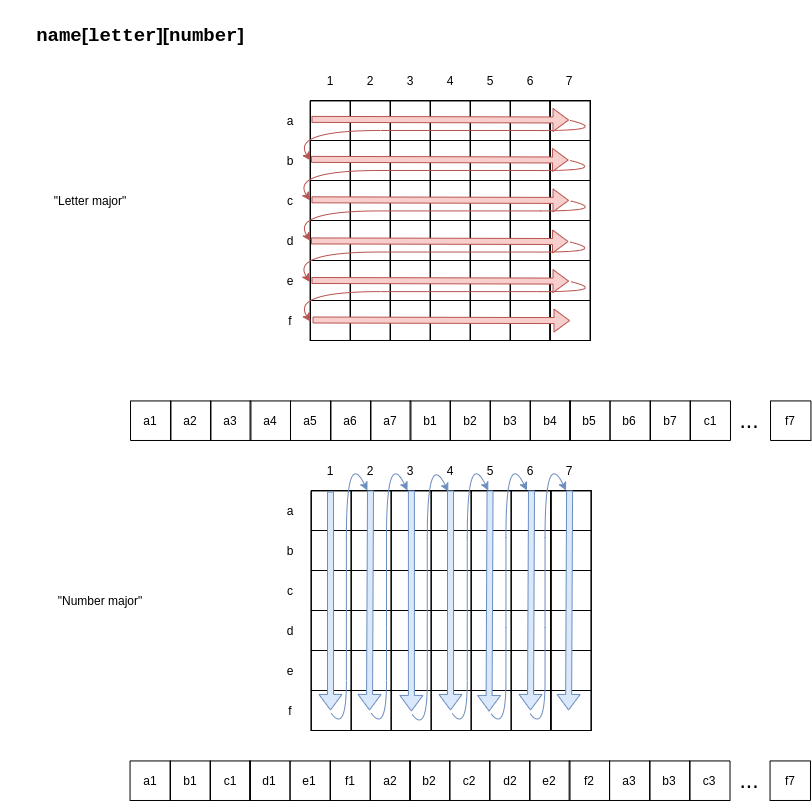
\includegraphics[width=\textwidth]{2.pdf}
\end{center}

\section*{2}
\label{sec:orgabe351b}
\begin{itemize}
\item Lower bound \(\ge 0\)
\item Lower bound \(\ge  support(AB) + support(AD) - support(A) = (3 + 2 - 5) = 0\)
\item Lower bound \(\ge support(AB) + support(BD) - support(B) = 3 + 0 -3 = 0\)
\item Lower bound \(\ge support(AD) + support(BD) - support(D) = 2 +0 - 2 = 0\)
\item Max(lower bound) = 0
\item upper bound \(\le support(AB) = 3\)
\item upper bound \(\le support(AD) = 2\)
\item upper bound \(\le support(BD) = 0\)
\item Min(upper bound) = 0
\item \(0 = 0\) so it is derivable
\end{itemize}
\end{document}
